\documentclass[12pt]{article}
%compile using XeLaTeX
\usepackage{diary_style}
\setlength{\footskip}{\paperheight
  -(0.75in+\voffset+\topmargin+\headheight+\headsep+\textheight)
  -0.75in}

%\fontspec{Times New Roman}

\DeclareMathOperator{\di}{d\!}
\newcommand*\Eval[3]{\left.#1\right\rvert_{#2}^{#3}}

\begin{document}

%\doublespacing
\vspace{1.0 \baselineskip}

\begin{flushright}
	Alexander Caines\\
	MATH-310\\
	3-29-2021\\
\end{flushright}

\begin{center}
	\textbf{\underline{EXAM 2}}
\end{center}


%\vspace{0.5 \baselineskip}

\begin{enumerate}
	\item[1.] The following are the results of running an ANOVA on the three factors (temperature, fabric denier, and air pressure) 
	at each of their respective three levels. \emph{I was not able to factor the data for Fabric, so I will provide the results for 
		temperature and pressure.} Note that as temperature increases, the affect on the response becomes
		 more significant as the p-value decreases. For pressure, the same phenomenon occurs. As the pressure increases, the p-value 
		decreases, and thus the significance of the affect increases. 
			\begin{figure}[!h]
				\centering
				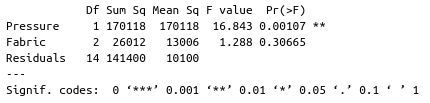
\includegraphics[width=8cm]{p1pics/8degrees.png}
				\caption{Results ANOVA at 17.2 kPa}
			\end{figure}
			\begin{figure}[!h]
				\centering
				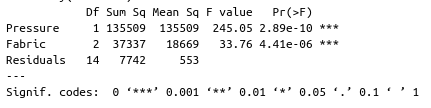
\includegraphics[width=8cm]{p1pics/50degrees.png}
				\caption{Results ANOVA at 34.4 kPa}
			\end{figure}
			\begin{figure}[!h]
				\centering
				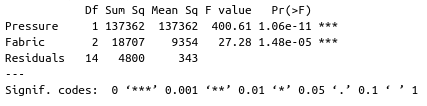
\includegraphics[width=8cm]{p1pics/75degrees.png}
				\caption{Results ANOVA at 103.4 kPa}
			\end{figure}
			\begin{figure}[!h]
				\centering
				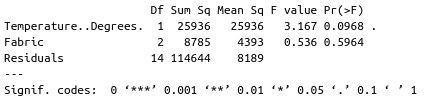
\includegraphics[width=8cm]{p1pics/17kPa.png}
				\caption{Results of ANOVA for temperature at 8 Degrees}
			\end{figure}
			\begin{figure}[!h]
				\centering
				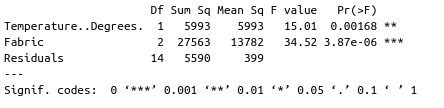
\includegraphics[width=8cm]{p1pics/34kPa.png}
				\caption{Results ANOVA for temperature at 50 degrees}
			\end{figure}
			\begin{figure}[!h]
				\centering
				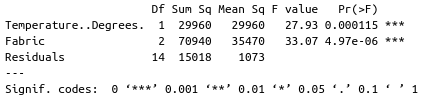
\includegraphics[width=8cm]{p1pics/103kPa.png}
				\caption{Results ANOVA for temperature at 75 degrees}
			\end{figure}
	\newpage
	\item[2.]
		\begin{enumerate}
			\item[(a)] Given that the points in the dataset (without having plotted them) seem to increase linearly when ordered, it seems as if the prices are deterministically related to the height.
			\item[(b)] The scatter plot indicates a positive, linear relatonship between height and price.
				\begin{figure}[!h]
					\centering
					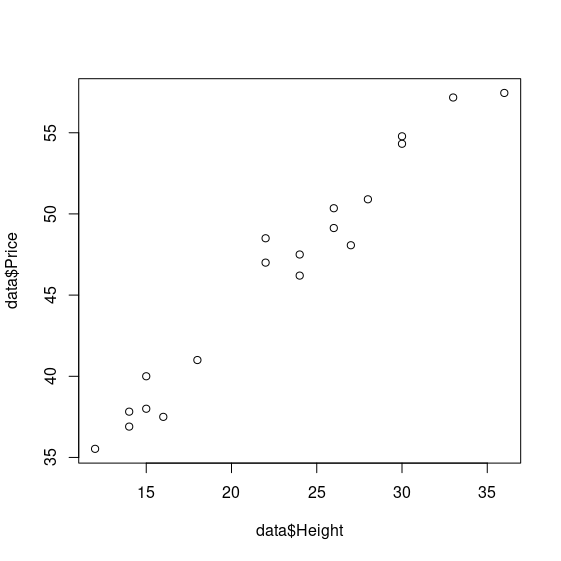
\includegraphics[width=8cm]{2b.png}
				\end{figure}
			\item[(c)] The equation of least squares is $y = 0.98715x + 23.77215$.
			\item[(d)] At a height of 27, the corresponding price is $\$50.43$. Given the summary below, the 
			corresponding residual is the result of the least squares (50.4252) plus the median residual (-0.8796), which is $49.55$.
				\begin{figure}[!h]
					\centering
					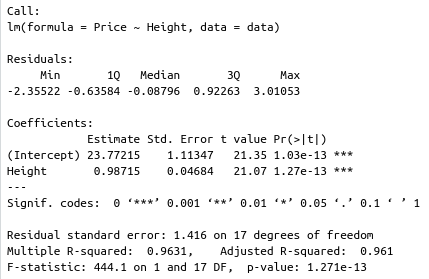
\includegraphics[width=8cm]{2d.png}
					\caption{Summary of linear model.}
				\end{figure}
			\item[(e)] In referring to the above figure, one will see that the adjusted R-squared is 0.96. So, 96\% 
			of the variation in sales price can be attributed to the approximate linear relationship 
			between truss height and price.
		\end{enumerate}
	\item[3.] 
		\begin{enumerate}
			\item[(a)] Below is the result of the following line of code, given the appropriate datset, $data$:
				$$model \leftarrow lm(NO3 ~ CO, data=data);\text{ } summary(model)$$ 
				\begin{figure}[!h]
					\centering
					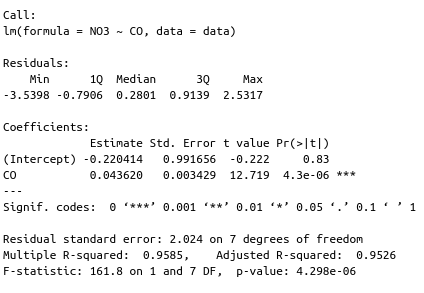
\includegraphics[width=8cm]{no3copmodel.png}
					\caption{Model of NO3 and CO data.}
				\end{figure}
			\item[(b)] The equation produced by the linear regression in R was 
$$\hat{y} = 13.63x + 21.97 $$ So, the prediction for
 $x=400$ is $5473.97$. Given that the mean of CO is $211.89$, the following work shows 
		that the prediction interval is $(-139.5264, 563)$.
			$$\hat{y} = mean(data\$CO);\text{ }t = 0.627;\text{ } error = 21.734;\text{ }r^2 = deviance(model)$$
			\item[(c)] Without the largest value of CO, the fitted equation is $\hat{y} = 15.21x + 21.70$, 
			yielding $6105.7$ as the prediction: a number far outside the previous interval. So, 
			the largest CO value has a substantial affect on the model.
		\end{enumerate}
	\item[4.] Below I show that $SSE = S_{yy} - \hat{\beta}_1S_{xy}$.
		\begin{center}
		\begin{math}
		\begin{aligned}
			SSE &= \sum{y^2_i} - \hat{\beta}_0\sum{y_i} - \hat{\beta}_1\sum{x_iy_i}\\
			&= \sum{y^2_i} - (\bar{y} - \hat{\beta}_1\bar{x})\sum{y_i} - \hat{\beta}_1\sum{x_iy_i}\\
			&= \sum{y^2_i} -\bar{y}\sum{y_i} + \hat{\beta}_1\bar{x}\sum{y_i} - \hat{\beta}_1\sum{x_iy_i}\\
			&= \sum{y^2_i} -\frac{1}{n}\sum{y_i}\sum{y_i} + \hat{\beta}_1(\sum\bar{x}{y_i} - \sum{x_iy_i})\\
			&= \sum{y^2_i} -\frac{1}{n}(\sum{y_i})^2 - \hat{\beta}_1((\sum{x_iy_i}) - \sum{\bar{x}y_i})\\
			&= S_{yy} - \hat{\beta}_1((\sum{x_iy_i}) - \sum{\bar{x}y_i})\\
			&= S_{yy} - \hat{\beta}_1S_{xy}\\
		\end{aligned}
		\end{math}
		\end{center}
	\item[5.] Although I was not able to format the data to run the ANOVAs properly, I would have gone about this 
		problem by running an ANOVA to see if there is any significant affect on setosa by any of the listed factors.
		If the ANOVA indicated that one of them did by, returning a p-value less than 0.05, then I would have run four pairwise t-tests to determine which one had the most significant affect. After determining this, I would have tested my assumptions by checking whether or not the dataset I was using satisifed homogeneity of variances. 
		in order to deter
\end{enumerate}

\end{document}
